\documentclass{beamer}
\usepackage{varioref}
%\usepackage[hidelinks]{hyperref}
\usepackage{cleveref}
\usepackage{tabu}
\usepackage{booktabs}
\usepackage{graphicx}
\newcommand{\story}[3]{\item As a #1, I want to be able to #2 so I can #3.}
\newcommand{\requirement}[1]{The system shall #1.}

\title{Use Cases\\
  {\large and}\\
  Functional Requirements}
\author{PolitiMap Team}

\begin{document}
\begin{frame}
  \maketitle
\end{frame}

\begin{frame}
  \centering
  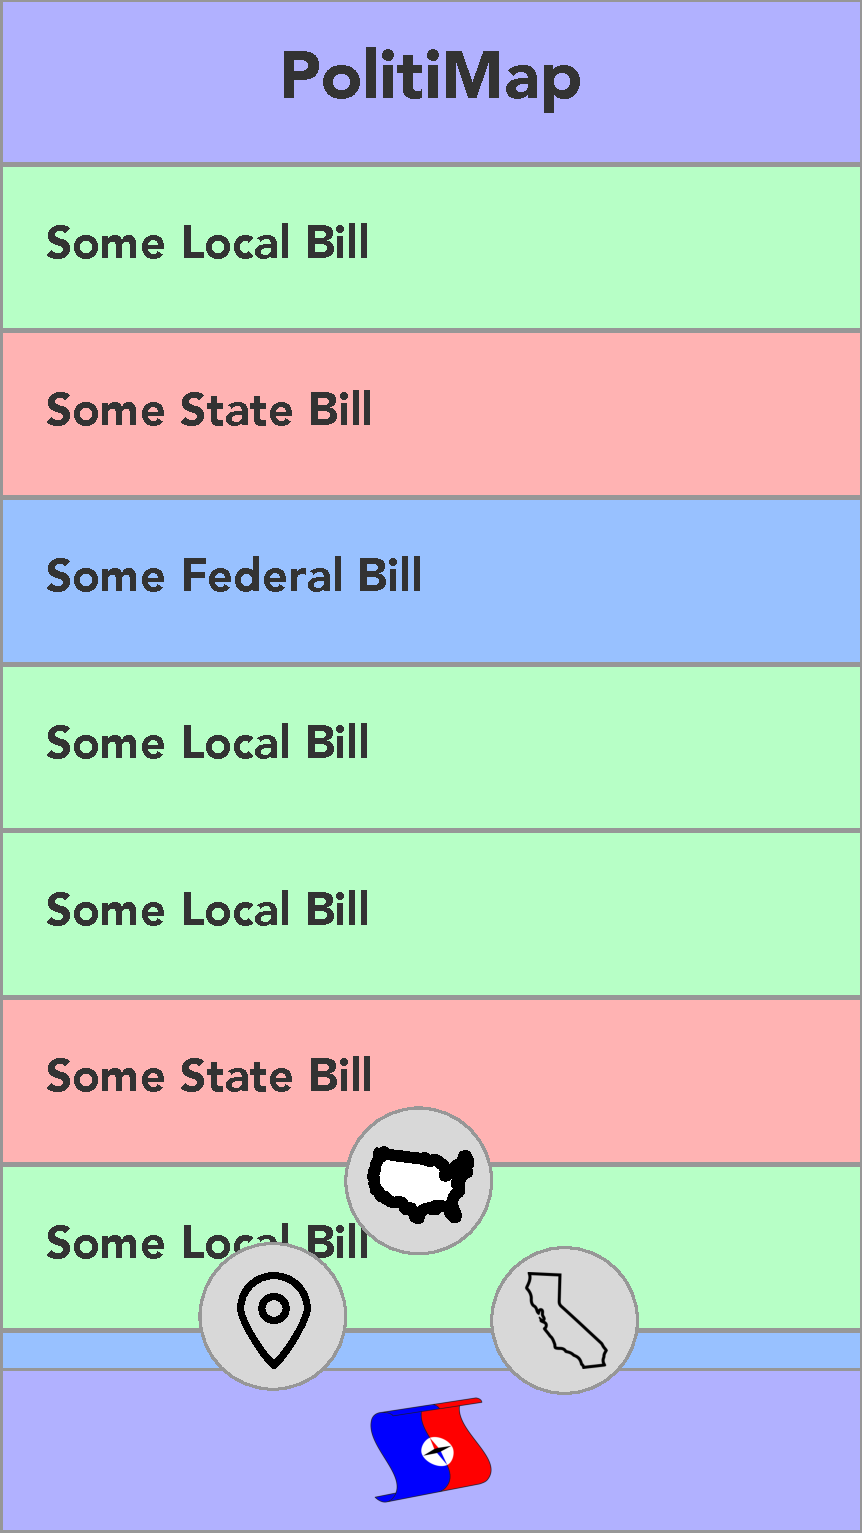
\includegraphics[height=\textheight,page=1]{UseCaseBoard.pdf}
\end{frame}
\begin{frame}
  \centering
  \includegraphics[height=\textheight,page=2]{UseCaseBoard.pdf}
\end{frame}
\begin{frame}
  \centering
  \includegraphics[height=\textheight,page=3]{UseCaseBoard.pdf}
\end{frame}
\begin{frame}
\begin{tabu}{rX}
Use Case Name:&View Federal Bills\\
Actors:&The Application User; The Swift iOS Application; The Backend Server\\
Description:&The application shall display a list of federal bills and further information about each upon selection.\\
Preconditions:&
\begin{enumerate}
\item The device is connected to the internet.
\item The backend is loaded with the organized data.
\item The device has the application downloaded, updated, and open to the home screen.
\item The backend server is running, whether it be an AWS component or EC2 instance.
\end{enumerate}\\
\end{tabu}
\end{frame}
  \begin{frame}
    \begin{tabu}{lX}
Postconditions:&
\begin{enumerate}
\item A list of federal bills will be shown and likely scrolled-down, or the details of a specific bill will be showing.
\item A request will have been made to the AWS component or EC2 instance.
\item TBD - The federal bills may be cached in the user's device.
\end{enumerate}
\end{tabu}
\end{frame}
  \begin{frame}
    \begin{tabu}{lX}
Normal Flow:&
\begin{enumerate}
\item The user chooses to view the list of bills relating to their local, state, and federal governments.
\item A GET request is made to the web server while the user sees a loading animation.
\item The user selects to filter the list of bills to show only federal bills.
\item The user scrolls through the bills and notices an interesting one.
\item The interesting bill is selected and the user reads related information, including a summary, associated representatives, and links to related external documentation.
\end{enumerate}
\end{tabu}
\end{frame}
  \begin{frame}
    \begin{tabu}{lX}
Alternative Flows:&
\begin{enumerate}
\item The user selects a federal bills list instead of filtering a combined list.
\item The bills are loaded upon opening the application and only refreshed manually.
\item The bill information does not include associated representatives.
\item The bill shows dynamic data, such as votes and comments.
\end{enumerate}\\
\end{tabu}
\end{frame}
  \begin{frame}
    \begin{tabu}{lX}
Exceptions:&
\begin{enumerate}
\item Unable to load the bills through the lack of an internet connection.
\end{enumerate}\\
Includes:&
\begin{enumerate}
\item An external library to make the GET request.
\end{enumerate}\\
Priority:&High - One of the core functions of the application.\\
Frequency of Use:&Depends on the number of users and other variables.\\
Special Requirements:&
\begin{enumerate}
\item The application requests the data asynchronously.
\item The device is an iPhone 5 or newer.
\item Specific bill information is loaded with a GET request after a bill is selected.
\end{enumerate}\\
Assumptions:&
\begin{enumerate}
\item Viewable federal bills exist in the backend.
\item Representatives have been linked to associated bills.
\item Documentation links have been added to associated bills.
\end{enumerate}
\end{tabu}
\end{frame}

\begin{frame}
  \frametitle{Functional Requirements}
  \begin{enumerate}
    \item The system shall store the frequently accessed data, such as the list of federal bills, in AWS S3, to minimize the cost to \$.004 per 10,000 requests.
    \item The system shall refresh the list of federal bills from GET requests through a network connection.
    \item The system shall default to sorting bills by the timestamp of their last update in content.
  \end{enumerate}
\end{frame}

\begin{frame}
  \frametitle{Non-Functional Requirements}
  \begin{enumerate}
    \item The system shall load the list of bills in under two seconds.
\item The system shall have zero memory leaks.
\item Federal bills shall be updated within one day of receiving new information.
  \end{enumerate}
\end{frame}

% Andrew
\begin{frame}
\begin{tabu}{rX}
  Use Case Name: & Display Agenda\\
  Actors: & The PolitiMap App\\
  Description: & Display the agenda for the next City Council meeting\\
  Preconditions: &
  \begin{enumerate}
  \item The user has chosen a location which has a city council
  \item The location is currently supported by the app
  \item The app is open
  \item The user has chosen ``City Council Meeting'' from the list of events.
  \end{enumerate} \\
  Postconditions: &
  \begin{enumerate}
  \item The app shows the agenda for the next City Council meeting for
    the selected location.
  \end{enumerate} \\
\end{tabu}
\end{frame}
\begin{frame}
  \begin{tabu}{rX}
  Normal Flow: &
  \begin{enumerate}
  \item The user opens app
  \item The app requests data from server
  \item (Alternative flow 1)
  \item The app displays a list of upcoming events
  \item The user chooses the City Council item
  \end{enumerate} \\
  Alternative Flows: &
  Alternative flow 1
  \begin{enumerate}
  \item Read data from cache
  \end{enumerate} \\
  Priority: & High\\
  Assumptions: & Council meeting agendas will be available for all
  supported locations\\
\end{tabu}
\end{frame}

\begin{frame}
  \frametitle{Functional Requirements}
  \begin{enumerate}
    \item \requirement{load data in the JSON format specified in
      an appendix}
    \item \requirement{fetch the data to load from the web}
    \item \requirement{only load JSON data for the locations selected}
  \end{enumerate}
\end{frame}

\begin{frame}
  \frametitle{Non-Functional Requirements}
  \begin{enumerate}
    \item \requirement{provide a button to add an event to the user's calendar}
    \item \requirement{display a list of upcoming meetings}
    \item \requirement{display the date and time of each meeting in the list of meetings}
    \item \requirement{display the location of each meeting in the list of meetings}
  \end{enumerate}
\end{frame}

% Yash
\begin{frame}
\begin{tabu}{rX}
  Use Case Name: & Save Locations\\
  Actors: & The PolitiMap App\\
  Description: & Save multiple locations on the home page of the Application\\
  Preconditions: &
  \begin{enumerate}
  \item The location is currently supported by the app
  \item The app is open
  \item The app is on the home page
  \end{enumerate} \\
  Postconditions: &
  \begin{enumerate}
  \item The app shows the saved location on the home page.
  \item The app should be able to access the location and show its Political information when tapped
  \end{enumerate}
\end{tabu}\end{frame}
  \begin{frame}\begin{tabu}{lX}
  Normal Flow: &
  \begin{enumerate}
  \item The user opens app
  \item The app loads locations saved by the user
  \item The user views saved locations
  \item (Alternative flow 1)
  \item The user searches a new locations
  \item The user chooses to save the location
  \end{enumerate} \\
  Alternative Flows: &
  Alternative flow 1
  \begin{enumerate}
  \item Save location
  \end{enumerate} \\
  Priority: & High\\
  Assumptions: & All locations can be found\\
\end{tabu}
\end{frame}

\begin{frame}
  \frametitle{Functional Requirements}
  \begin{enumerate}
\item \requirement{Alter order of saved addresses}
\item \requirement{Delete addresses the user doesn't want anymore}
\item \requirement{Edit saved addresses}
  \end{enumerate}
\end{frame}

\begin{frame}
  \frametitle{Non-Functional Requirements}
  \begin{enumerate}
    \item \requirement{securely store the saved addresses}
    \item Memory should be available to store the local addresses
    \item Home page should be loaded instantly with the static information
  \end{enumerate}
\end{frame}

% Jason
\begin{frame}
\begin{tabu}{rX}
  Use Case Name: & View bills that affect foreign students\\
Actors: & \begin{enumerate}\item iOS Application
    \item The back-end server
\end{enumerate} \\
  Preconditions: &
  \begin{enumerate}
    \item The device is connected to the internet and the app is downloaded.
    \item The app is opened showing the main page.
  \end{enumerate} \\
  Postconditions: &
  \begin{enumerate}
    \item One of the menus should direct the user to a new
      page.
    \item The page will contain bills that are related to foreign students.
  \end{enumerate} \\
\end{tabu}
\end{frame}

\begin{frame}
  \frametitle{Functional Requirements}
  \begin{enumerate}
    \item The system will have a drop-down menu to display
      Bills related to foreign students.
    \item The system will save recently viewed Bills.
    \item The system will allow the users to call their city
      council by pressing the contact button.
  \end{enumerate}
\end{frame}

\begin{frame}
  \frametitle{Non-Functional Requirements}
  \begin{enumerate}
    \item UI is easy to follow for the users.
    \item Pages are loaded in less than 2 seconds
    \item The system will show a loading bar when pages are
      loading.
  \end{enumerate}
\end{frame}

\begin{frame}
\begin{tabu}{rX}
  Use Case Name: & Display Policy Positions\\
  Actors: & The PolitiMap App\\
  Description: & View policy summary of given local politician on active issues\\
  Preconditions: &
  \begin{enumerate}
  \item The user's location is currently supported by the app
  \item The user has chosen the city council member to evaluate
  \item Push
  \item The user has selected "Policy Positions" from menu options
  \end{enumerate} \\
  Postconditions: &
  \begin{enumerate}
  \item The app displays a summarized list of policy positions on active local legislation, and
  	lists a "position not available" message if position is indeterminate
  \end{enumerate} \\
\end{tabu}
\end{frame}
  \begin{frame}
    \begin{tabu}{lX}
  Normal Flow: &
  \begin{enumerate}
  \item The user opens the app
  \item The user specifies their location, or a cached location is processed
  \item The user selects "Politicians" from the lower UI menu
  \item The user selects their chosen politician from the "Your Representatives" list
  \item The user navigates to "Policy Positions" using the UI menu
  \end{enumerate} \\
  Priority: & Medium\\
  Special Requirements: & None\\
  Assumptions: & Policy positions will be available publicly through government or council member's website\\
\end{tabu}
\end{frame}

\begin{frame}
  \frametitle{Functional Requirements}
  \begin{enumerate}
    \item \requirement{load data in the JSON format specified in
      an appendix}
    \item \requirement{fetch the data using AJAX or other method of web request}
    \item \requirement{only load JSON data for the locations selected
      by the user}
    \item \requirement{data on politicians must be verifiable and completely accurate}
  \end{enumerate}
\end{frame}

\begin{frame}
  \frametitle{Non-Functional Requirements}
  \begin{enumerate}
    \item \requirement{provide menu UI on politician page for ease of navigation}
    \item \requirement{display bulleted list of policy positions on active legislation}
  \end{enumerate}
\end{frame}
\end{document}
